% Document class
\documentclass[titlepage]{report}

% Packages
\usepackage{lipsum,eurosym,enumitem,multicol,hyperref,geometry,graphicx,float,listings}
\usepackage[utf8]{inputenc}
\usepackage[T1]{fontenc}
\usepackage[dvipsnames]{xcolor}
\usepackage[french]{babel}
\usepackage{subfig}
\usepackage{listings}
\usepackage{qrcode}
\usepackage{ragged2e}
\usepackage{tikz}
\usepackage{graphicx}
\usepackage{subcaption}

% Document geometry
\geometry{paper=a4paper,textwidth=16cm}

% Definition of \maketitle
\title{Projet de Programmation Java : MoonQuest}
\author{Par : Lucien Piat \\ \vspace{.5cm} Sous la direction de : Karkar Slim}
\date{Avril 2024}

\makeatletter         
\def\maketitle{
\raggedright
\begin{center}

\includegraphics[width = 0.5\textwidth]{img/logo_ub.png}\\[15ex]
{\Huge \bfseries \@title }\\[10ex] 
{\huge  \@author}\\[10ex] 
{\Large \@date}\\
\end{center}}
\makeatother


% Debut du Document
\begin{document}
\maketitle
\thispagestyle{empty} 
\newpage
\tableofcontents
\thispagestyle{empty} 

%Debut du sujet 
\pagenumbering{arabic}
\justify 

\chapter{Introduction}
\pagenumbering{arabic}
Java est un langage de programmation orienté objet qui permet de produire des applications sécurisées et qui offre une portabilité avancée du code grâce à une machine virtuelle.\\

Lors de ce projet de programmation, je développerai le jeu "MoonQuest" grâce à cet outil.  Cela me permettra de découvrir de nombreuses facettes du langage et me forcera à manipuler un projet complexe avec rigueur.\\

\begin{quotation}
    \textit{PS. Pour avoir une bonne expérience en lisant ce rapport, il est conseillé de lancer le .jar présent sur la page \href{https://github.com/Lucien-Piat/MoonQuest}{GitHub} et de laisser jouer les IA entre eux en partie rapide.}
\end{quotation}

\vspace*{2cm}
\begin{figure}[h]
    \centering
    \begin{tikzpicture}
        \node[anchor=south west,inner sep=0] (image) at (0,0) {
\includegraphics[width=0.4\textwidth]{img/moon_quest_logo.PNG}};
        \draw[line width=2pt, black] (image.south west) rectangle (image.north east);
    \end{tikzpicture}
\end{figure}

\chapter{Analyse du Sujet}

En lisant le sujet, nous allons essayer de déterminer quels seront les principaux challenges à décortiquer lors de l’implémentation de notre jeu.

\section{Les Pièces}
Le jeu MoonQuest est présenté sous la forme d'un échiquier sur lequel des pièces sont placées. Ces dernières sont des candidates parfaites pour être codées par des classes en Java. Ainsi, nous essaierons de réduire au maximum les répétitions de code en créant un maximum de sous classes pour généraliser les objets manipulés.

\section{Le Plateau et les Cases}
Le plateau de jeu sera formé de cases qui contiendront des pièces ou non. Nous pourrons aussi créer un clase Case qui nous permettra de généraliser la production de ces dernières. Un des enjeux est de faire apparaître ces cases sous forme de plateau à l'écran. Ce plateau, devra s’actualiser à chaque tour pour permettre au joueur de consulter l’avancement de la partie. 

\section{Les Règles de Déplacement}
De nombreuses règles sont présentes dans le jeu, il faudra les implémenter sous forme de méthodes() qui seront contenues dans les sous classes. L’utilisation de super() nous permettra de moduler la réponse des méthodes en fonction de la sous classe utilisée.

\section{La Création des Modes de jeu et des Joueurs}
Il sera aussi nécessaire de créer des joueurs IA pour effectuer des déplacements sur le plateau automatiquement. Leur nombre devra être modulable pour permettre à l’utilisateur de choisir entre un 1 contre 1, un jeu contre l’IA ou simplement regarder des IA s’affronter.\\

D'autre part, nous aurons besoin des menus pour permettre au joueur d’interagir avec le programme, donner la case à jouer, et paramétrer la partie. 

\section{L’initialisation de la Partie}
Grace à l’interaction du joueur avec les menus, il faudra créer une partie correspondant à ses choix. Il sera aussi nécessaire de placer toutes les pièces sur le plateau, aléatoirement pour les nuages et de façon déterminée pour les autres. 

\section{Le Tour par Tour}
Enfin, nous implémenterons dans une classe Main, toutes les boucles qui appellent les différentes méthodes pour le bon déroulement de la partie. Elles devront solliciter les joueurs à leur tour un par un. 

\section{La Fin de Partie}
En fin de partie, il faudra arrêter le jeu et déclarer un vainqueur. De plus, comme stipulé dans la consigne, tous les coups des joueurs devront être affichés pour résumer la partie. Cela implique de consigner chaque tour dans un cahier de log. 

\section{Les Extensions}
Notre jeu devra implémenter deux des trois extensions obligatoires parmi : 

\begin{itemize}[label=$\bullet$]
    \setlength\itemsep{1em}
    \item La surcharge de ressources,
    \item La grille infinie,
    \item Et la Sauvegarde. 
\end{itemize}

\chapter{Solutions Envisagées}
Avant de développer le jeu, j’ai passé un long moment pour déterminer la façon la plus efficace et simple de le coder. Comme nous allons le voir par la suite, cela fut un échec sur certains points. 

\section{Pou les Extensions}
Le choix des extensions est crucial, car les trois propositions peuvent changer radicalement la façon de coder le jeu. J’ai donc décidé de choisir celles qui, à mon sens, étaient les plus simples à implémenter, soit la grille infinie et la surcharge de ressources.\\

J’ai réalisé plus tard que la surcharge de ressources était en réalité un cauchemar à implémenter, car elle implique énormément de vérifications et de contraintes auquel je n’avais pas pensé (pour en citer : la superposition de deux pièces avec des couleurs différentes, la suppression des pièces au sein du vecteur empêche la lecture, le changement dynamique de la taille de la police pour accommoder plusieurs pièces…)

\section{Pour l’Affichage}
Afin de pousser le projet au bout, j’ai décidé de faire un affichage graphique dans une fenêtre à part du terminal. Pour ce faire, je voulais utiliser la bibliothèque Swing qui gérait la création de fenêtres.  En actualisant le contenu de cette dernière à chaque tour, je pourrais avoir un affichage dynamique du jeu.\\

Après avoir déjà réalisé des affichages de plateaux de jeu dans un terminal au semestre dernier. J’ai voulu m’éloigner de ce mode de fonctionnement archaïque qui est très rébarbatif dans la conception. D’autre part, Java est un langage originellement développé pour les applets qui semblent très adapté à ce genre d’affichage graphique simple. \\

Ainsi, je comptais créer une classe Plateau qui entendrait la classe Jframe pour stocker les cases.

\section{Pour le Plateau}
Le plateau sera donc une Jframe contenant un vecteur. Ce dernier contiendra des objets de la classe Case qui étendra la classe Jlabel. Les Jlabel sont des classes qui peuvent être placées dans les Jframe. Elles peuvent prendre des couleurs différentes, contenir des chaînes de caractères et, en étendant la classe, nous pourrons aussi ajouter d’autres variables intéressantes comme un vecteur contenant les pièces sur la case.  \\

Afin de faciliter la lecture du jeu, les cases qui sont situées sur la première ligne et la première colonne, ne contiendront qu’un caractère indiquant le nom de la ligne/colonne. Cela permettra au joueur de savoir les coordonnées de la pièce qu’il souhaite déplacer.  \\

Les cases jouables seront créées à l’initialisation du plateau dans le constructeur en alternant leurs couleurs. Toutes les cases contiendront une chaîne de caractère contenant leur nom, par exemple, la case sur la deuxième ligne, deuxième colonne sera ‘B2’. 

\section{Pour les Pieces}
La classe abstraite Piece sera la base pour la construction de tout le système, elle contiendra la plupart des méthodes pour nécessaires au mouvement de toutes les pièces du plateau. \\

On créera ainsi des sous classes pour les glaces, les nuages et les véhicules. Comme les différentes pièces ne sont pas soumises à des règles identiques, les méthodes qu’elles contiennent ne renvoient pas exactement les mêmes résultats. 

\section{Pour les Joueurs}
Initialement, je comptais créer une classe Tour qui appelle les différents intervenants dans la partie et qui gère les Pieces inertes. Comme nous le verrons, cette idée fut rapidement abandonnée. \\

De plus, il sera aussi nécessaire de construire un log qui sera affiché à la fin de la partie. Ainsi, je comptais profiter de la classe tour pour faire une pierre de coup, et, tout en gérant le bon déroulement de la partie inscrire les opérations dans ce dernier. 

\chapter{Algorithmes Choisis}
\begin{figure}[h]
    \centering
    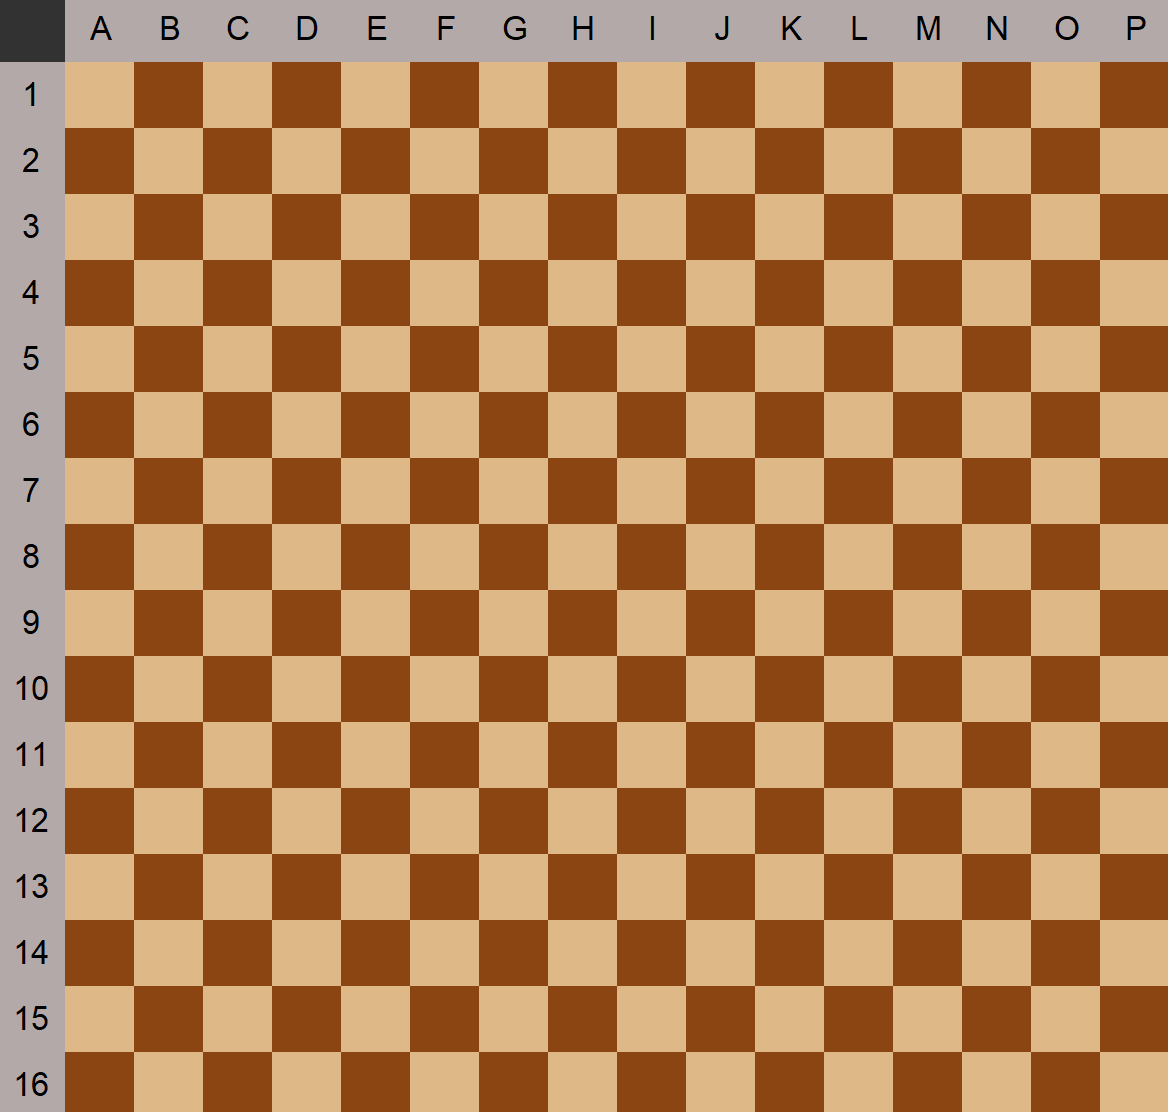
\includegraphics[width=0.5\textwidth]{img/plateau_vide.PNG}
    \caption{Exemple de plateau vide}
\end{figure}

Après une longue réflexion, j’ai commencé à me pencher sur le code en lui-même. Après avoir codé pendant plusieurs heures, j’ai fait face à un mur. En effet, placer les instances de Pièces à l’intérieur même des cases du plateau rend très compliquée l’interaction entre ces dernières. 

\section{Pour les Pieces}
Les pièces sur le plateau sont toutes issues de la classe abstraite Piece. Elles peuvent êtres initialisées dans des sous classes pour changer leurs comportement dans le jeu. \\

\begin{figure}
    \centering
    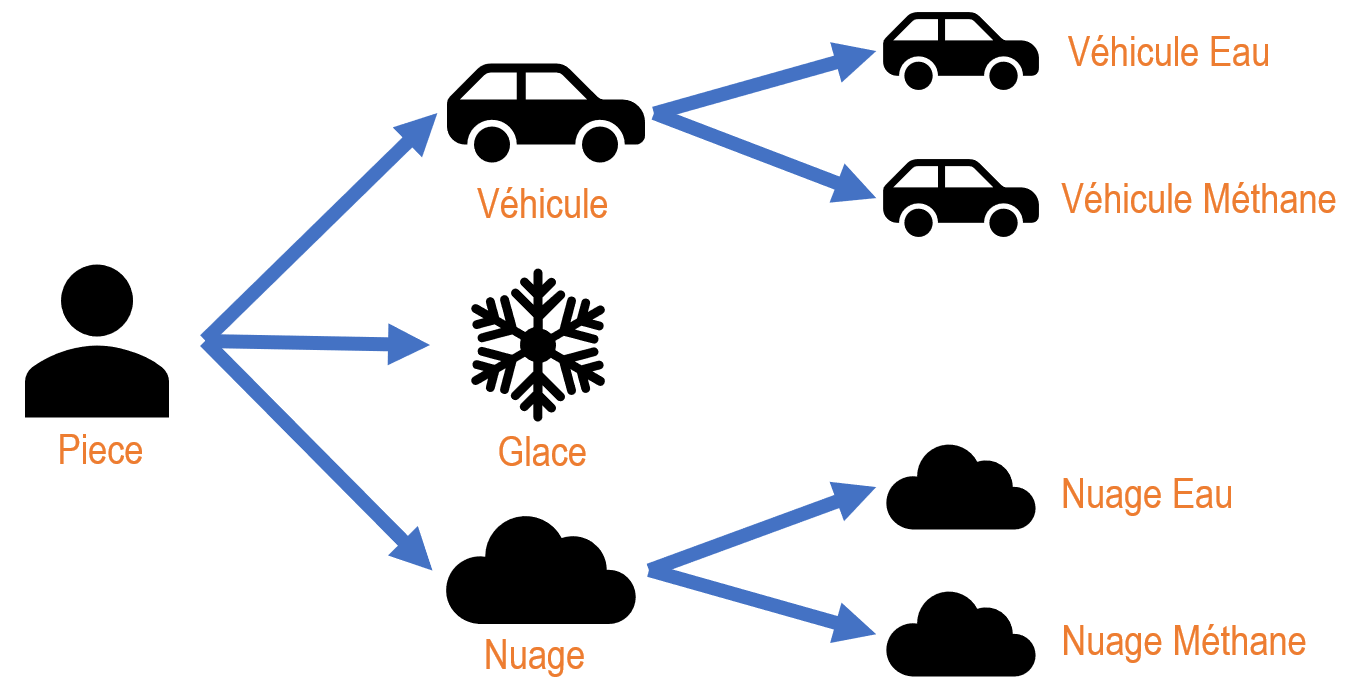
\includegraphics[width=0.5\textwidth]{img/schema_cases.PNG}
    \caption{Diagramme présentant les différentes instances de la classe Piece}
\end{figure}

\begin{samepage}
\noindent De plus elles possèdent plusieurs variables essentielles :\\
\begin{itemize}[label=$\bullet$]
    \setlength\itemsep{1em}
    \item La variable « player » prend la forme d’une couleur (package Color) et nous permet de connaître deux informations en même temps. Le plateau logique se servira de la couleur pour déterminer à quel joueur la pièce appartient elle. Le plateau graphique récupérera la couleur et affichera la pièce avec cette dernière.
    \item La variable curCase est une chaîne de caractères qui indique le nom de la case sur laquelle la pièce se trouve. 
    \item La variable toPrint indique une chaîne de caractères qui informera le plateau graphique de ce qu’il doit afficher dans la case.  
\end{itemize}
\end{samepage}

Ces trois variables sont présentes dans toutes les pièces. La classe Véhicule implémente aussi la variable capture qui a pour max 3 et qui est incrémentée à chaque fois que le véhicule détruit un nuage de son type. Cette variable est privée ce qui implique que si le véhicule disparaît, ses points de captures sont définitivement perdus. \\

Les différentes instances des sous classes Pieces modulent la façon dont elles répondent aux méthodes. Par exemple, quand on demande à une pièce dans quelle direction elle souhaite bouger, en fonction de son type le traitement de la demande variera comme suit : 
\begin{figure}
    \centering
    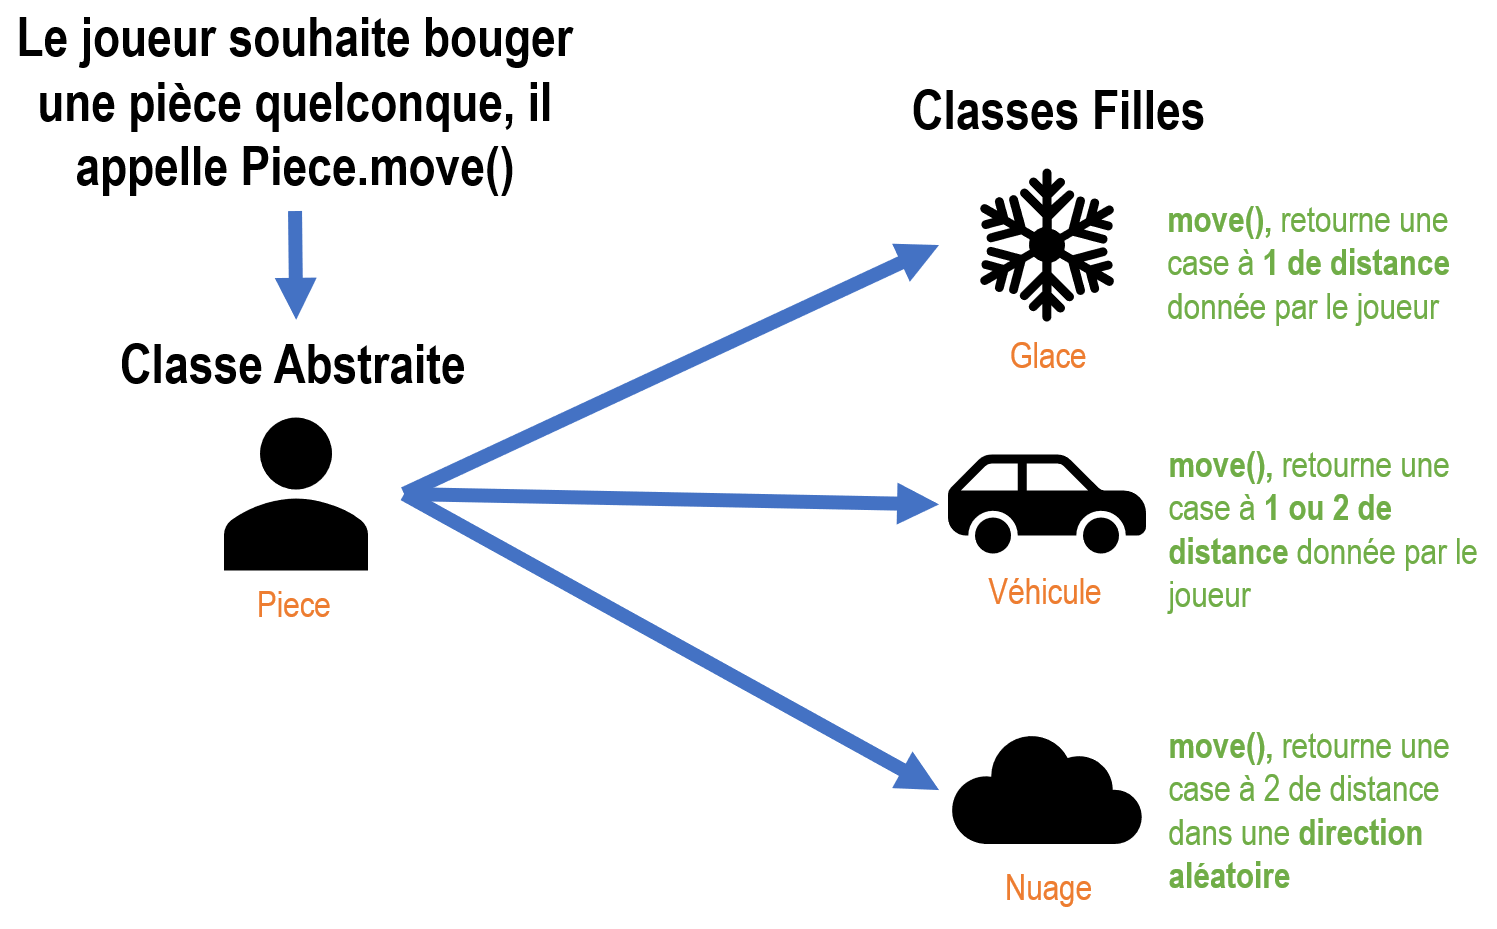
\includegraphics[width=0.5\textwidth]{img/schema_move.png}
    \caption{Diagramme présentant les différentes méthodes move()}
\end{figure}
Comme chaque pièce nous informe de la case sur laquelle elle se situe et non l’inverse, on a une dissociation entre la logique et le graphique. En effet, afin de savoir si une destruction doit avoir lieu, il suffit de savoir si la case de destination d’une pièce qui souhaite bouger est déjà présente chez une autre. Si oui, il suffit d’appliquer les règles entre les deux pièces concernées. \\

Toutes les pièces sont stockées dans un vecteur et initialisées au sein de la classe PlateauLogique. Quand un nouveau plateau logique est créé, son constructeur appelle des méthodes d’initialisation des différents types de cases qui sont générées en suivant le schéma dicté dans le sujet. 

\section{Pour l’Affichage du Plateau et des Cases}
\subsubsection{Les Cases Jouables}
Ainsi, j’ai donc complétement modifié mon code pour séparer le plateau logique qui contient les pièces et le plateau graphique qui contient les cases. \\

Après chaque coup, le plateau graphique accède au contenu du plateau logique qui stocke un vecteur de pièces. Après avoir nettoyé toutes les valeurs des cases, il commence à les remplir. \\

Chaque case stocke les informations qui permettent de déterminer à quoi elles ressemblent. Outre la couleur du fond, on lui attribue une chaine de caractères correspondant à la concaténation du nom de toutes les pièces qui lui sont liées. Afin de gérer la surcharge de ressources, on divise la taille de la police en fonction du nombre de caractères. Finalement, on détermine la couleur de la police. Si, toutes les pièces contenues appartiennent au même joueur, ou qu’une pièce est seule, la case hérite de leurs couleurs. Sinon, afin d’éviter les incompréhensions, en cas de discorde sur la couleur des pièces présentent, le noir est choisi. \\

Une fois paramétrées, toutes les cases qui sont en réalité des Jlabel sont placées dans l’ordre sur le plateau qui est en réalité une Jframe. 
\subsubsection{Les Cases non Jouables}
Il existe quelques cases non jouables sur le plateau, elles servent uniquement de repère pour le joueur, et affichent leurs noms seulement. Pour ne pas les mettre à jour et éviter qu’elles se fassent nettoyer avant chaque coup, on leur attribue un booléen isSide. Si isSide est « true », alors la case esquivera toutes les méthodes de mise à jour.   
\begin{figure}[h]
    \centering
    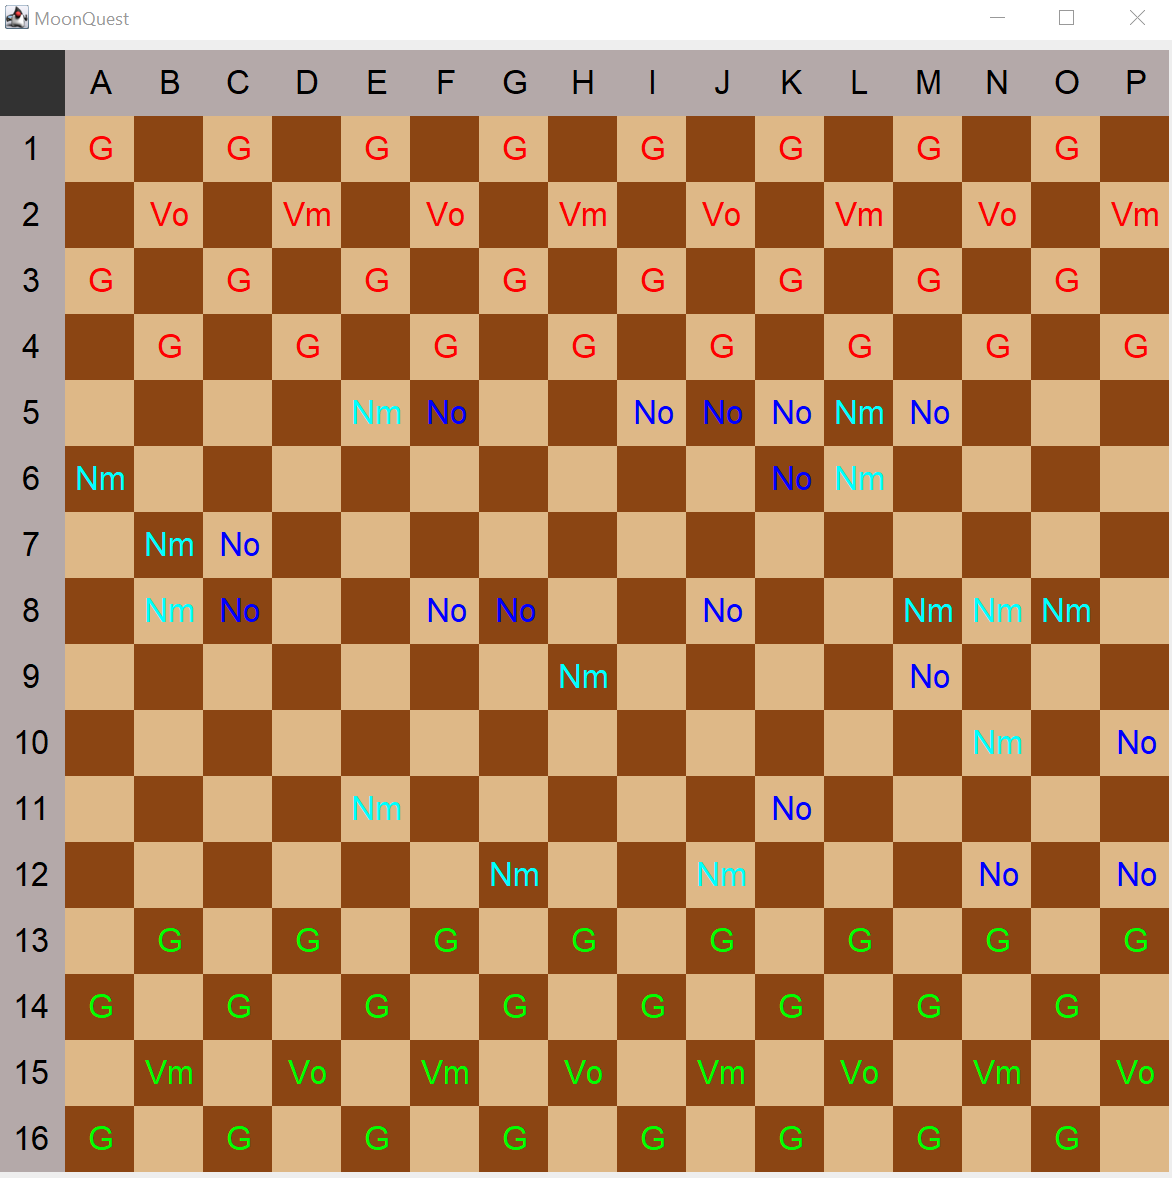
\includegraphics[width=0.5\textwidth]{img/plateau.PNG}
    \caption{Exemple de plateau après initialisation}
\end{figure}

\section{Pour les Règles de la Partie. }
La plupart des contraintes des règles de la partie sont implémentées dans des vérifications au sein de la classe PlateauLogique. 
\noindent Voici le déroulement d’un déplacement classique sur le plateau :
\begin{itemize}[label=$\bullet$]
    \setlength\itemsep{1em}
    \item On demande à une Piece la direction vers laquelle elle souhaite se déplacer. Si la pièce répond, on récupère la direction et sa variable currCase.
    \item Comme la variable currCase est construite de cette façon : colonne + ligne par exemple « C13 » on divise la chaîne de caractères en deux « C » et « 13 ». 
    \item Dans deux listes triées, sont stockés les différents noms de colonnes et de lignes. Ainsi, on récupère l’indice de la ligne et de la colonne de la case dans les listes. Par exemple « C » = 2 et « 13 » = 12. 
    \item Si la direction choisie est Ouest par exemple, il suffit de prendre comme case de destination la case a l’indice -1 de l’indice de la case actuelle. Comme ceci, on peut déterminer que la case de destination est B13 dans l’exemple. On utilise le même principe pour le déplacement Nord Sud mais avec les nombres.  Autre exemple, la pièce souhaite aller au Nord-Est. On découpe la chaine en deux C et 13. On prend l’indice -1 de 13 pour aller au Nord et l’indice +1 de C pour aller à l’Est. On reconstruit la chaîne et on détermine que la case de destination porte de nom D12. 
    \item Maintenant que nous possédons la case de destination de la pièce, il est temps d’appliquer les règles. Si aucune autre pièce ne se situe sur la case on associe à la pièce sa nouvelle position. Sinon, on vérifie l’instance de la pièce qui se déplace et de la ou les pièces déjà présentes. On appelle la méthode qui permet de gérer notre cas de figure et si une ou des pièces doivent être détruites on les ajoute temporairement au vecteur toDestroy.
    \item Finalement, on applique la destruction. La destruction est appliquée à la fin, car il est impossible de parcourir le vecteur contenant toutes les pièces tout en l’éditant. La surcharge de ressources impose ce genre de tampon.  
\end{itemize}
Après avoir réalisé la manipulation, on peut terminer le tour. Si le déplacement est aérien, on fait deux fois le déplacement d’affilé pour parcourir deux cases en un tour. Cependant, à la place de déplacer la pièce dans la case la plus proximale, on vérifie juste qu’aucune glace ne soit présente pour empêcher le mouvement. Si non, on déplace la pièce dans la case la plus distale. 

\section{Pour les Joueurs}
Comme énoncé plus haut, les joueurs étaient initialement codés directement dans le main de mon programme. Cependant, il est complexe de gérer la création de la partie dynamiquement en fonction du choix du type de jeu (vs IA, vs Joueur…). Ainsi, j’ai décidé de créer une autre famille de classe, les Joueurs. Il existe trois sous types de joueurs qui implémentent tous la méthode joue() mais y répondent différemment quand elle est appelée :
\begin{itemize}[label=$\bullet$]
    \setlength\itemsep{1em}
    \item La sous classe JoueurIA sélectionne une de ses pièces aléatoirement et un nombre aléatoire. Ce nombre aléatoire servira d’indice pour sélectionner une direction dans un vecteur contenant tous les déplacements possibles.   
    \item La sous classe JoueurHumain la plus complexe, implémente toutes les méthodes qui interpellent le joueur quand c’est son tour.
    \item La sous classe JoueurNuages permet de résoudre le problème du déplacement des nuages. Elle appellera tous les nuages présents dans le vecteur des pièces et les fera bouger aléatoirement comme décrit dans le sujet. 
\end{itemize}
Les méthodes qui interpellent le joueur sont sous forme de popup de Jframe. Voici la liste des pop-ups et leurs rôles. 
\begin{figure}[h]
    \centering
    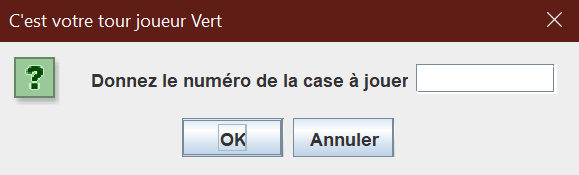
\includegraphics[width=0.5\textwidth]{img/votre_tour.PNG}
    \caption{Elle permet au joueur d’entrer une chaîne de caractères qui correspond au nom d’une case et de valider. Si le joueur entre une case qui ne contient pas une de ses pièces ou une case qui n’existe pas, la méthode réouvre le popup. On appelle la méthode move() de la pièce qui se trouve dans la case sélectionnée. }
\end{figure}

\begin{figure}[h]
    \centering
    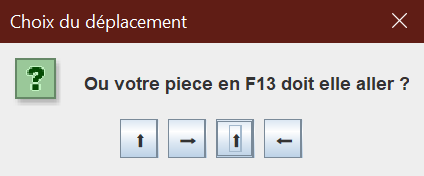
\includegraphics[width=0.4\textwidth]{img/simple_move.PNG}
    \caption{Si le déplacement est terrestre, le joueur peut directement cliquer sur une flèche pour le déplacement.}
\end{figure}

\begin{figure}[h]
    \centering
    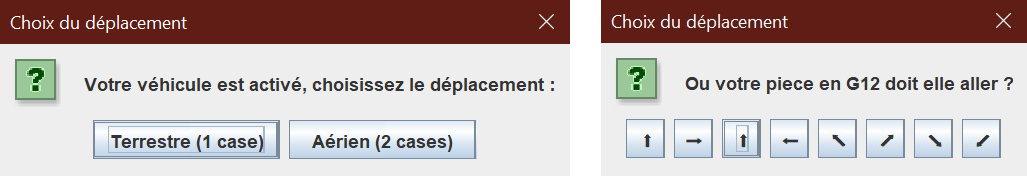
\includegraphics[width=0.9\textwidth]{img/choix_vol.png}
    \caption{Dans le cas où la pièce sélectionnée est activée, le joueur peut choisir entre le déplacement terrestre ou aérien. S’il sélectionne le vol, un menu contenant plus de directions s’ouvre.}
\end{figure}

\section{Pour le Log de la partie}
\begin{figure}[h]
    \centering
    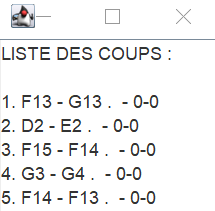
\includegraphics[width=0.2\textwidth]{img/log.PNG}
    \caption{Le Logger}
\end{figure}
Les logs de la partie sont gérés par une classe Logger. Elle contient un vecteur de chaînes de caractères. A chaque nouvelle entrée, on parcoure le vecteur de pièces pour calculer les captures de chaque joueur, puis on ajoute le dernier mouvement au log. Ce mouvement est renvoyé par les différents Joueurs en sortie de la méthode joue(). Ainsi, quand un joueur a fini son tour on actualise le Logger. Il est bon de noter que les mouvements des nuages ne sont pas loggés pour améliorer la lisibilité de ce dernier.\\

Comme le Logger possède toutes les informations de la partie à chaque tour, on implémente une méthode qui lui permet de savoir si la partie est terminée ou pas. Si oui elle renvoie un booléen vrai. Dans ce cas-là, la partie s’arrête et un popup de fin apparaît.\\

Pour améliorer la lecture du jeu, on affiche le Logger pendant toute la partie grâce à une JTextArea. 

\section{Pour les Extensions}
Ce n’est que, bien avancé dans le développement du jeu, que je me suis rendu compte de l’erreur que j’avais fait de choisir la surcharge de ressources. Il a fallu faire en sorte de créer un buffer pour la modification des pièces dans le vecteur qui les contient. Sans cela, impossible de le parcourir pour vérifier si deux pièces se trouvent sur la même case. \\

D’autre part, la coloration et la police de la case sont dynamiques pour autoriser plusieurs pièces à entrer dans la case sans se superposer. Ce choix m’a fait perdre plusieurs heures à coder dans les méthodes les cas où les pièces sont sur la même case. \\

Pour le plateau infini, cela fut beaucoup plus simple. Lors du déplacement, quand la chaîne de caractères indiquant le nom de la case est découpée si l’indice demandé est au bout du plateau, on le remet à 0.

\section{Pour le Programme Principal}
\noindent Finalement, le programme principal permet de lancer une partie. \\

Tout d’abord il demande au joueur de sélectionner le mode de jeu et de créer deux sous classes de Joueur en fonction de son choix. Ensuite, il initialise un joueurNuage, un Logger, un plateauGraphique et un plateauLogique. Sauf contre-indication du Logger, il appelle la méthode tour() qui fait jouer chaque joueur un par un jusqu’à la fin de la partie.  

\chapter{Au-delà du Code}
En plus du code lui-même, de nombreux outils ont été découverts lors de ce projet. Ces derniers ont largement participé au bon déroulement du travail et ont leur place dans ce rapport. 
\section{La GUI}

\includegraphics[width=0.05\textwidth]{img/vscode_logo.png}\\

\href{https://code.visualstudio.com/}{Visual Studio Code} a permis d’éviter de nombreuses prises de têtes grâce à la coloration de la syntaxe, le formatage automatique, et l’autocomplétion des méthodes. Sans lui, ce projet aurait vite viré au cauchemar. 
\section{Le Versioning}

\includegraphics[width=0.05\textwidth]{img/github_logo.png}\\

Grace à\href{https://github.com/}{GitHub}, le suivi du travail et la création du code fut relativement simple. Il a notamment permis de travailler sur plusieurs machines lors des nombreux déplacements ce semestre. 
\section{Le Framework}

\includegraphics[width=0.1\textwidth]{img/maven_logo.png}\\

\href{https://maven.apache.org/}{Le Framework Maven} a permis de faciliter la gestion de la forme du programme grandement. L’outil fut découvert par hasard lors de recherches bibliographiques sur Java. 
\section{La Documentation}
Grace au livre « \href{https://babordplus.hosted.exlibrisgroup.com/primo-explore/fulldisplay?vid=33PUDB_UB_VU1&id=991003988839704672&inst=33PUDB_UB&context=L}{Programmer en Java} » de Claude Delannoy, disponible à la bibliothèque universitaire ce projet a pu être développé avec les bonnes pratiques de java en tête. La bibliothèque Swing été facilement apprise et de nombreuses bases ont été approfondies. 

\chapter{Conclusion}    
Lors de ce projet, de nombreux problèmes se sont présentés auquel il a fallu trouver des solutions. J’ai découvert un bon nombre d’outils qui seront utiles pendant toute ma vie de bio-informaticien. \\

Afin de finaliser ce travail, j’ai généré une Java-doc complète, un fichier .jar pour tester le programme facilement, ainsi qu’une page GitHub pour le partage du projet. \\

Bien que très satisfait du travail que j’ai produit, si le temps ne manquait pas, voici les éventuelles améliorations que j’aurais apporté au programme : 

\begin{itemize}[label=$\bullet$]
    \setlength\itemsep{1em}
    \item La sauvegarde de la partie en cours. Cela aurait pu être facilement fait en exportant le plateau logique. 
    \item Des logos pour les pièces auraient été bien plus lisibles que les lettres et couleurs actuelles. 
    \item Une vraie IA qui ne fait pas des coups au hasard rendrait le jeu plus intéressant. 
    \item Finalement le Drag and Drop est probablement ce qui manque le plus à ce jeu. En effet, le fait de pouvoir directement prendre les pièces et les déplacer sur la case souhaitée aurait été plus facile pour le jouer. Malheureusement, la documentation que j’ai utilisé pour Swing n’aborde pas ce sujet. 
\end{itemize}
Finalement, en regard du nombre d’heures que j’ai passé à coder un simple plateau d’échec. Il m’est désormais plus facile d’apprécier le temps de développement qui a dû être injecté sur d’autres jeux codés en Java comme Minecraft. La charge gargantuesque de travail que représente un système aussi complexe m’impressionne. 

\begin{figure}[h]
    \centering
    \qrcode{https://github.com/Lucien-Piat/MoonQuest}
    \caption{Le GitHub du projet}
  \end{figure}

\end{document}


